\documentclass[a4paper]{article}

\usepackage{polski}
\usepackage[utf8]{inputenc}
\usepackage{amsmath}
\usepackage{graphicx}
\usepackage[colorinlistoftodos]{todonotes}

\usepackage{float}

\usepackage{listings}

\title{Opis zadania 8.1}

\author{Przemysław Sagało}

\date{\today}

\begin{document}
\maketitle
\section{Specyfikacja problemu}   
Rozwiązanie równania liniowego:
\begin{equation}
a \cdot x + b \cdot y+c = 0 
\end{equation} 
zależy od wartości współczynników $a$, $b$ i $c$.
Powyższe równanie możemy rozwikłać, tak aby wartość $y$ wyznaczana była w sposób bezpośredni:
\begin{equation}
\label{eq:form2}
y = - \frac{a}{b} x - \frac{c}{b}.
\end{equation}
Taka postać równania wymusza aby $b \neq 0$.
\newline
Gdy $a=0$ równanie \ref{eq:form2} przyjmuje postać:
\begin{equation}
y = - \frac{c}{b}.
\end{equation}
Z kolei gdy $c=0$ równanie \ref{eq:form2} ma postać:
\begin{equation}
y = - \frac{a}{b} \cdot x.
\end{equation}

\section{List kroków}
\begin{enumerate}
\item Sprawdź czy $b=0$. Jeżeli tak to należy zakończyć program i np. zwrócić wyjątek, jeżeli nie idź dalej,
\item jeżeli $a=0$ i $c=0$, to $y=0$,
\item jeżeli $a=0$, to $y = - \frac{c}{b}$,
\item jeżeli $y = - \frac{a}{b} \cdot x$,
\item z kolei w ostatnim kroku sprawdzamy ostatnią możliwość czyli $a \neq 0$ i $b \neq 0$ i $c \neq 0$ co daje rozwiązanie w postaci: $y = - \frac{a}{b} x - \frac{c}{b}$.
\end{enumerate}

\section{Schemat blokowy}
\begin{figure}[H]
	\begin{center}
		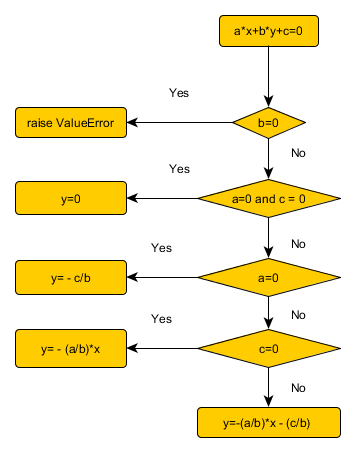
\includegraphics[width=11cm]{block_diagram.png}
		\caption{Schemat blokowy powyższego zagadnienia.}
	\end{center}	
\end{figure}

\section{Schemat w postaci drzewa}
\begin{figure}[H]
	\begin{center}
		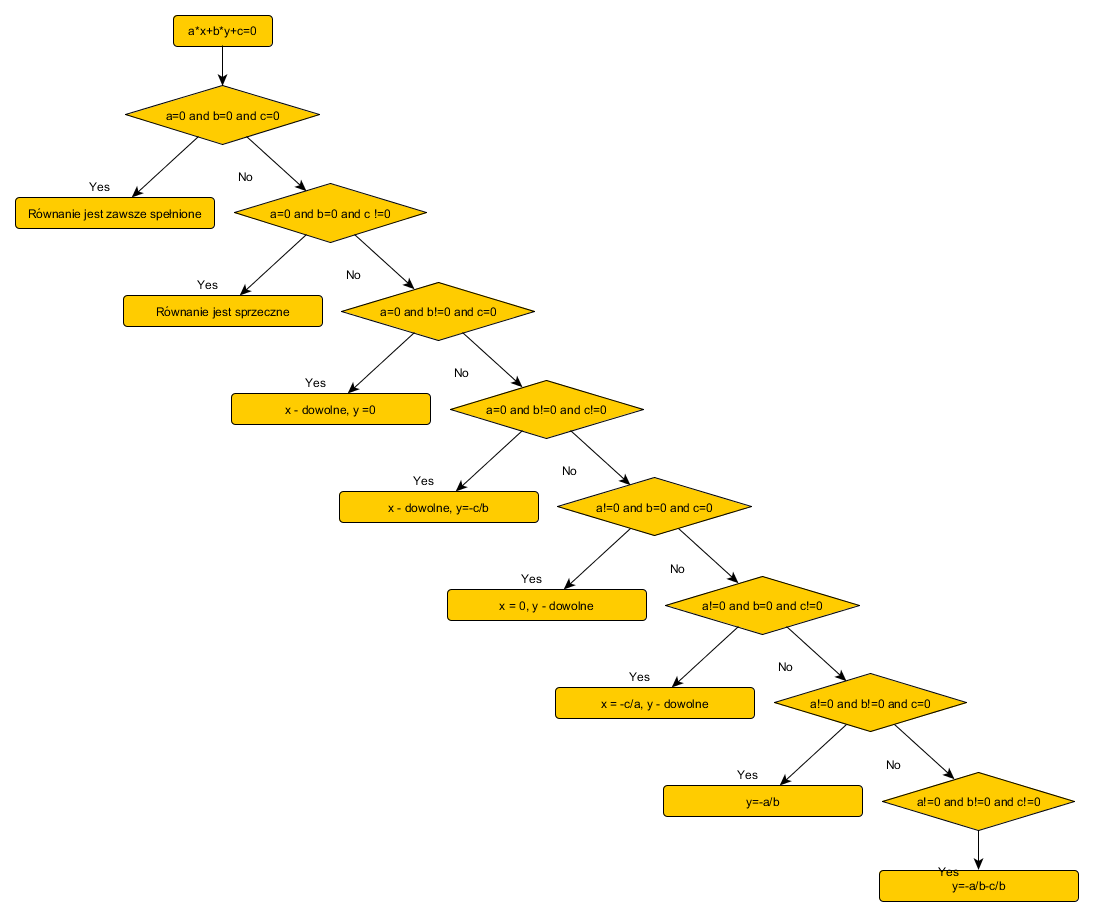
\includegraphics[width=15cm]{tree_diagram.png}
		\caption{Schemat w postaci drzewa dla powyższego zagadnienia.}
	\end{center}	
\end{figure}
\newpage

\section{Algorytm}
\begin{lstlisting}[language=Python]
def solve1(a, b, c):
    """Rozwiazywanie rownania liniowego a x + b y + c = 0."""
    if b == 0:
        raise ValueError('b nie moze byc rowne 0')
    else:
        if a == 0 and c == 0:
            to_return = 'y=0'
        elif a == 0:
            to_return = 'y={}'.format(-c / float(b))
        elif c == 0:
            to_return = 'y={}*x'.format(-a/float(b))
        else:
            to_return = 'y={0}*x{1}'.format(-a/float(b), -c/float(b))

    return to_return
\end{lstlisting}

\end{document}